\documentclass[12pt, a4paper]{scrreprt}

\renewcommand*\familydefault{\sfdefault} 
%\usepackage[T1]{fontenc}

\usepackage[english]{babel}
%\usepackage{cite}
\usepackage[utf8]{inputenc}
%\usepackage[onehalfspacing]{setspace}
\usepackage{geometry, textcomp}
\newgeometry{right=2cm,left=4cm, top=2.5cm, bottom=2.3cm, footnotesep=0.5cm}
%\usepackage[acronym]{glossaries}

\usepackage[printonlyused]{acronym}  % Abkürzungsverzeichnis [nur verwendete Abkürzugen]

%\glsenablehyper

%\makeglossaries

\usepackage{savesym}
\usepackage{amsmath,amssymb,amstext}
%\usepackage{graphics}
\savesymbol{iint}
\usepackage{txfonts}

\restoresymbol{TXF}{iint}
\usepackage[automark,headsepline,ilines,komastyle]{scrpage2}
\usepackage{blindtext}
\usepackage[euler]{textgreek}
\setlength{\parindent}{0pt}
\setlength{\headheight}{1.5\baselineskip}
\renewcommand{\baselinestretch}{1.5}

\pagestyle{scrheadings}
\clearscrheadfoot
\ihead[]{}
\chead[]{}
\ohead[]{\headmark \hfill \thepage}
\ifoot[]{}
\cfoot[]{}
\ofoot[]{}

\setheadsepline[\textwidth]{1pt}
\usepackage{tabularx}
\usepackage{colortbl}
\usepackage{multirow}
\usepackage{hhline}
\usepackage{array}
\usepackage{tocloft}
\usepackage[hidelinks]{hyperref}
\tocloftpagestyle{scrheadings}
\renewcommand{\chapterpagestyle}{scrheadings}
\usepackage[font=footnotesize]{caption}

\usepackage{tikz}
\usepackage{rotating} 

\newenvironment{packed_item}
	{\begin{itemize}
			\setlength{\itemsep}{0pt}
			\setlength{\topsep}{0pt}
			\setlength{\parsep}{0pt}
			\setlength{\parskip}{0pt}}
		{\end{itemize}}
	
\usepackage[style=authoryear, natbib=true, backend=biber]{biblatex}

\renewcommand{\nameyeardelim}{ }
\usepackage[babel,german=guillemets]{csquotes}

\makeatletter

\newrobustcmd*{\parentexttrack}[1]{%
	\begingroup
	\blx@blxinit
	\blx@setsfcodes
	\blx@bibopenparen#1\blx@bibcloseparen
	\endgroup}

\AtEveryCite{%
	\let\parentext=\parentexttrack%
	\let\bibopenparen=\bibopenbracket%
	\let\bibcloseparen=\bibclosebracket}

\makeatother

\usepackage{pstricks}
\usepackage{pstricks-add}

\bibliography{Lit.bib}

\usepackage[final]{pdfpages}

\begin{document}
		\begin{titlepage}
			\begin{center}
			%\setlength{\headheight}{1.5\baselineskip}
			\renewcommand{\baselinestretch}{1.5}
					\textbf{\large FOM - Hochschule für Oekonomie \& Management \\
						Hamburg \\
						\ \\
						Master-Studiengang Big Data \& Business Analytics \\
						3. Semester \\
						\ \\
						Development of a system to control and monitor blood pressure \ \\
						measurements to prevent cardiovascular disease \ \\
						\ \\
						}
						
					\textrm{
						\ \\
						Betreuer: Prof. Dr. Kai Brüssau \\
						\ \\
						Autor: Jacqueline Franßen \\
						\ \\
						Matrikel-Nr: 496804 \\
						\ \\
						3. Fachsemester \\
						\ \\
						Hamburg, den 29.02.2020 \\
						}
			\end{center}
		\end{titlepage}

%\includepdf{Image/Deckblatt.pdf}

			\setcounter{tocdepth}{3}
			\setcounter{secnumdepth}{3}		
			\pagenumbering{Roman}
			\thispagestyle{empty}
			\pdfbookmark{\contentsname}{toc}\tableofcontents
			\newpage
			\listoffigures
			\listoftables

			\pagenumbering{arabic}
			\thispagestyle{empty}
\chapter{Abstract}\label{abstract}

This scientific article focusses on the development of a chatbot and the analysis of blood pressure measurements.
The main purpose of this scientific article is to develop...
This can lead to...
What is more, .... 
The first business case is that...
Second,. 
Furthermore, ...
Third,...
Fourth,...
Last, ...

\chapter{Introduction}\label{introduction}

\section{Problem statement}
According to....
Another problem are 
All of these use cases can be automated and implemented by an application....

\section{Aim and scope of this work}
%describe aim
The first aim of this scientific work is to develop a solution ...
%describe scope
What is important, the developed model is only a reference model....

\chapter{Fundamentals}\label{fundamentals}

\section{Related Work}

\section{Current algorithms, solutions to predict metastasis}

\section{Overview: Apps to predict metastasis}

\footnote{\cite{vijini_gen_alg}}


\chapter{Functionality of XXX, YYY}
Here all used algorithms and patterns shall be explained

\section{Technology XXX}
\section{Technology YYY}


\chapter{Analysis and Development}

\section{User Research}

\subsection{User interviews}
\subsection{What is important? - Relevant features}
\subsection{How can processes be improved?}


\section{Development of system to predict metastasis and recidives} 

\section{Data Research}
\section{\ac{CRISP-DM}: Model Planning and Learning}
\section{Testing}
\section{Results} 

\chapter{Results}
\section{Validation of results}
\section{Limitation in the development process}

\chapter{Conclusion and Outlook}
\section{Conclusion}
\section{Outlook}


\chapter{Abbreviations}
\begin{acronym}[CRISP-DM]
\acro{crisp-dm}[CRISP-DM]{CRoss-Industry Standard Process for Data Mining}
\acro{cfo}[CFO]{Chief Financial Officer}
\acro{who}[WHO]{World Health Organization}
\acro{iarc}[IARC]{International Agency for Research on Cancer}
\acro{ham10000}[HAM10000]{Human Against Machine with 10000 training images}
\end{acronym}

\printbibliography[heading=bibintoc]

\chapter{Appendix A}\label{appendix a}
\ohead[]{Ehrenwörtliche Erklärung \hfill \thepage}

\null\vfill
\textbf{Ehrenwörtliche Erklärung}

Hiermit versichere ich, dass die vorliegende Arbeit von mir selbstständig und ohne unerlaubte Hilfe angefertigt worden ist, insbesondere dass ich alle Stellen, die wörtlich oder annähernd wörtlich aus Veröffentlichungen entnommen sind, durch Zitate als solche gekennzeichnet habe. Ich versichere auch, dass die von mir eingereichte schriftliche Version mit der digitalen Version übereinstimmt. Weiterhin erkläre ich, dass die Arbeit in gleicher oder ähnlicher Form noch keiner Prüfungsbehörde / Prüfungsstelle vorgelegen hat. Ich erkläre mich damit nicht einverstanden, dass die Arbeit der Öffentlichkeit zugänglich gemacht wird. Ich erkläre mich damit einverstanden, dass die Digitalversion dieser Arbeit zwecks Plagiatsprüfung auf die Server externer Anbieter hochgeladen werden darf. Die Plagiatsprüfung stellt keine Zurverfügungstellung für die Öffentlichkeit dar.

\ \\ \ \\ 


Ort, Datum (Vorname Nachname)

\vfill
\chapter{Appendix B}\label{appendix b}
%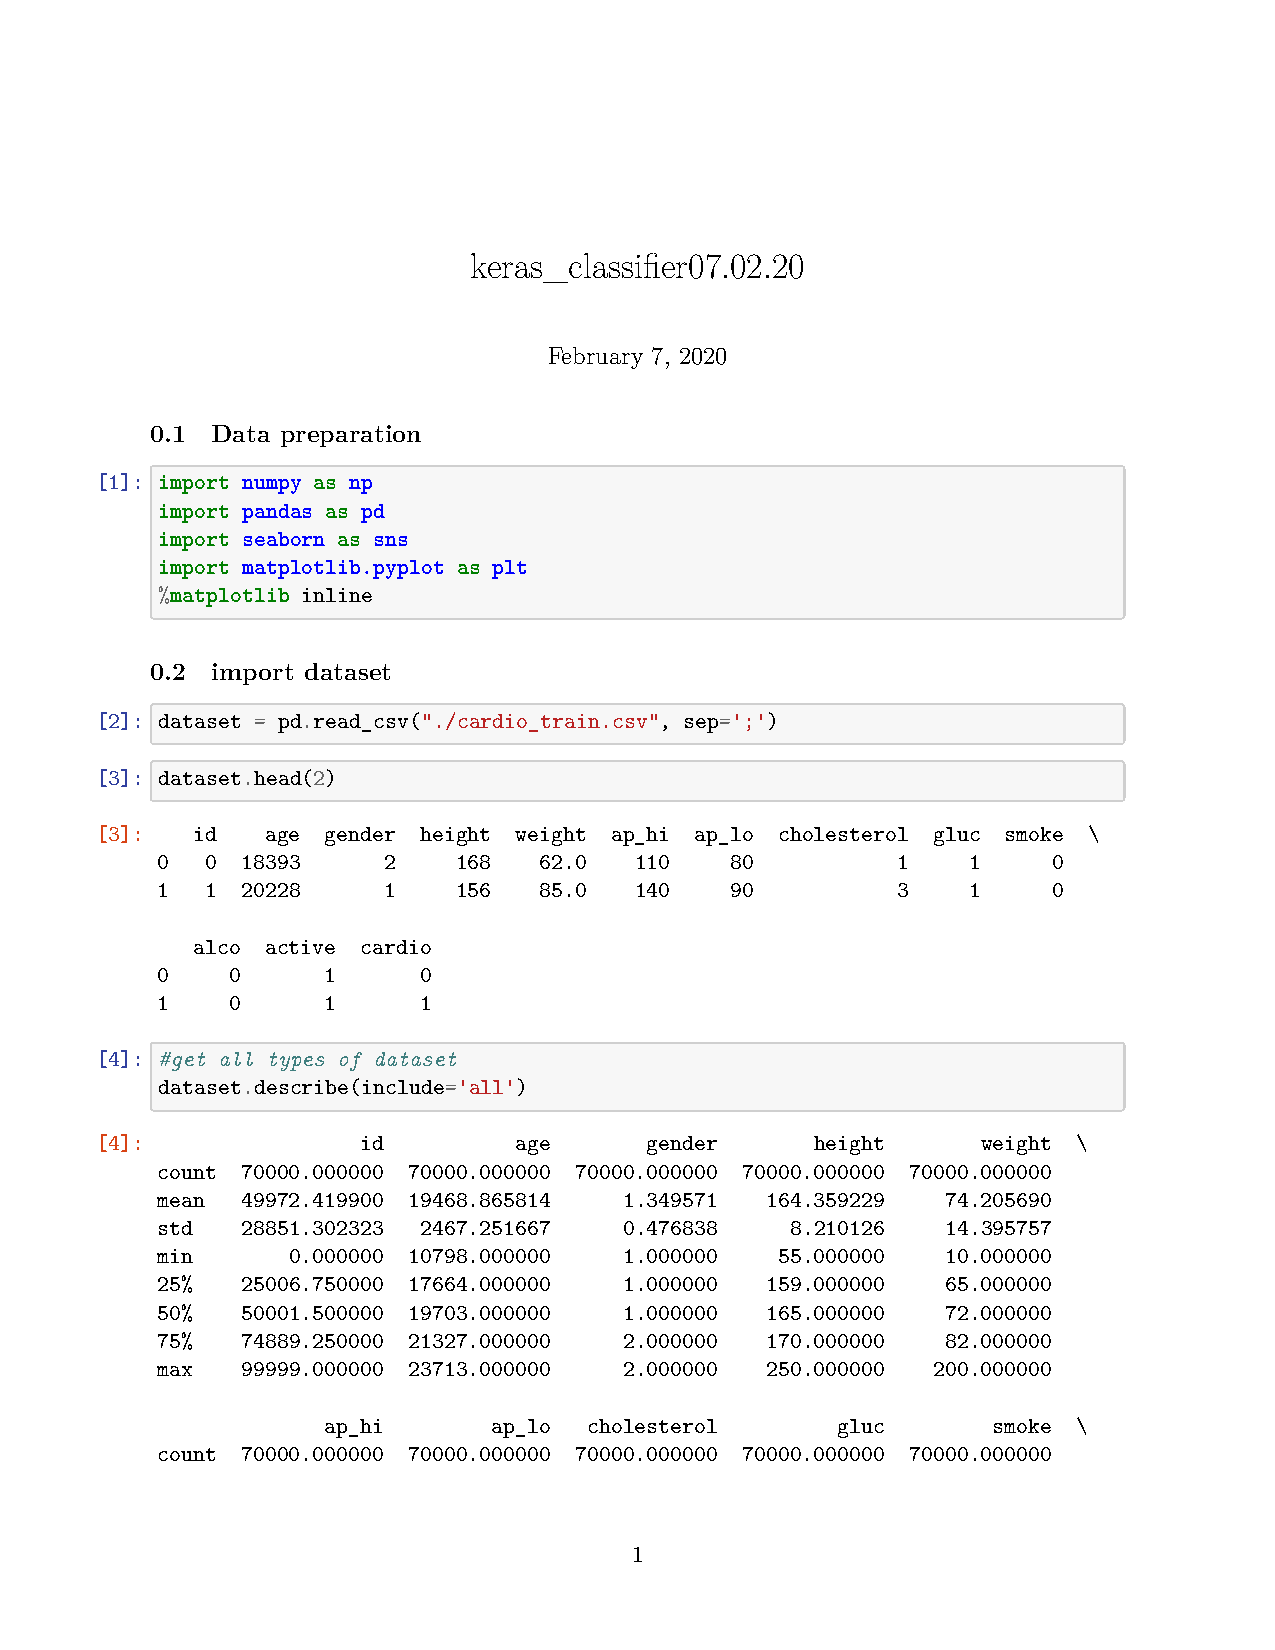
\includepdf[pages=-]{keras_classifier.pdf}

\end{document}
